\documentclass[../Main.tex]{subfiles}

\begin{document}
\author{Momentum of a Photon} %use author for title of lesson
\date{NOT ASSESSED} %use date to refer to topic in main booklet

\section{Momentum of a Photon} %Section is the title of the lesson repeated, ready for the main contents page.

\begin{frame}{Einstein's Energy-mass Equivalence}
    You will have heard by now of Einstein's most famous equation:

    \begin{equation*}
        E=mc^2
    \end{equation*} 

    where E is energy (J), m is mass (kg) and c is the speed of light.
\newline \newline
It means that for a very large amount of energy, mass can be created - or destroyed to release energy. This is the principle behind nuclear reactors and many aspects of particle physics -- as you shall see next year.
\newline \newline
Because of the huge amounts of energy involved, we typically only think of this for very small amounts of mass - on the order of the mass of an electron ~$10^{-30}kg$. %\pause

\begin{exampleblock}{You try}
What amount of energy would you need to create a single electron with mass $9.11\times 10^{-31}$kg? %\pause
--$8\times 10^{-14}$J.
\end{exampleblock}
In electronvolts this is equivalent to 500keV.
\end{frame}

\begin{frame}{A new unit for mass}
    In the world of the very small, it is much better to consider the mass in terms of the amount of energy required to produce this mass. 
\newline \newline
If we use $E=mc^2$, we can rearrange for
\begin{equation*}
    m=E/c^2
\end{equation*} and so if we take c to just be a constant with no value, and take energy in MeV we essentially get a unit of mass in 

\begin{equation*}
    [MeV]/[c^2]
\end{equation*} or units $MeV/c^2$ %\pause
\newline \newline
Hence we can say the mass of the electron is in fact $0.5MeV/c^2$
\end{frame}

\begin{frame}{Momentum?}
    But where does momentum fit into this? \newline \newline
    We know that anything with mass has momentum, equal to the product of the mass and velocity. If we consider that `c' is also technically a velocity, we now see that momentum has units

    \begin{equation*}
        [MeV]/[c]
    \end{equation*} %\pause

    But now we must consider the photon -- a photon has no mass, and should technically also have no momentum...
\end{frame}

\begin{frame}{Einstein's equation}
    $E=mc^2$ is not actually the full picture -- but merely only applies for a particle that is at \emph{rest}. This is why on your data sheet you are given a `rest' mass. %\pause

    \begin{equation*}
        E^2 = (mc^2)^2+(pc)^2
    \end{equation*}
    where E,m,c are as before, and p is the momentum. %\pause
    \newline \newline
    We see that if an object has no mass (only possible for photons/light), then it will have a momentum $p=E/c$.
    \newline \newline
Now we can take the energy of the photon using $E=hf$ and use this to find the momentum of the photon.
\begin{exampleblock}{Momentum of a gamma-ray photon}
    Taking the Planck constant to be $4.14\times 10^{-21}$MeVs, find the momentum in MeV/c of a photon of frequency $2\times 10^{19}$Hz %\pause
    -- 0.08MeV/c (or 80keV/c)
\end{exampleblock}
\end{frame}

\begin{frame}{Momentum of a photon}
    Now we can see that a photon can indeed have momentum, while also having no mass. This does not apply to us in real life, but means that photons can exert a pressure when reflecting off a surface -- recall Newton's second law in terms of momentum? %\pause

    \begin{equation*}
        F=\frac{\Delta p}{\Delta t}
    \end{equation*}

    Since $\Delta p$ is just $2p$ (photons reflect with the same velocity) -- and due to the quantum nature, the reflection occurs near-instantaneously (on a human scale anyway), the force exerted is \emph{relatively} large. 
\end{frame}

\begin{frame}{Applications -- solar sails}
    We humans cannot feel this force -- it is simply too small, but on the quantum scale, enough photons reflecting off a surface will induce a signficant acceleration, even for a `large' mass. This is the principle behind the solar sail, a new method developed to propel spacecraft and has been proven to work.

\begin{figure}
    \centering
    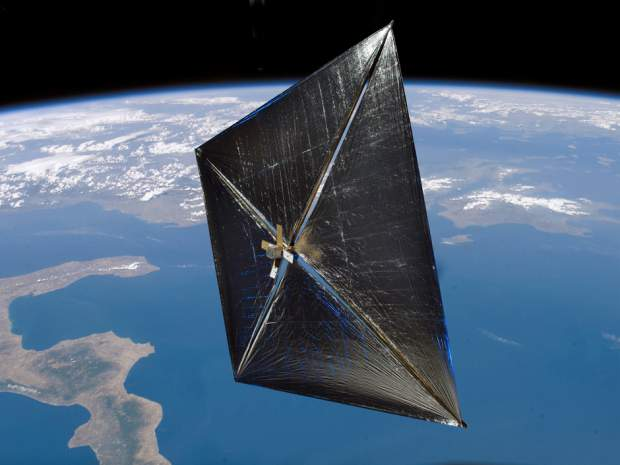
\includegraphics[height=3cm]{Quantum_Images/solarsail.png}
\end{figure}

We have a miniature version of this here in class -- which we can power using a laser.
\end{frame}

\end{document}